\chapter{Métodos e Desenvolvimento}
\label{cap:desen}
Este capítulo descreve as etapas de desenvolvimento e as metodologias empregadas neste trabalho. Buscaram-se estratégias sem intrusão ou grandes modificações nas políticas de escalonamento já implementadas pelo \textit{framework}. Nas Seções \ref{sec:collector} e \ref{sec:zookeeper} são apresentados em maior detalhe os coletores de contexto e a ferramenta de comunicação distribuída utilizados neste trabalho, respectivamente. Finalmente, na Seção \ref{sec:solucao} explica-se em profundidade a solução implementada neste trabalho e as justificativas para as decisões tomadas.

%-------------------------------------------------------------------
\section{Coletores de Contexto}
\label{sec:collector}
Após um estudo aprofundado dos escalonadores do Hadoop, ficou claro que o Capacity Scheduler já está estruturado de maneira a oferecer escalabilidade e um desempenho satisfatório. Porém, este escalonador possui um ponto fraco, o qual é exposto quando utilizado em um ambiente compartilhado. O Capacity Scheduler só recebe informações sobre os Node Managers no momento da inicialização destes, e ainda, a informação é obtida de um arquivo de configuração. A importância de que as informações sobre os Node Managers estejam atualizadas decorre da dependência intrínseca do escalonamento com a disponibilidade de recursos, na qual uma informação errada pode influenciar o algoritmo de maneira prejudicial e diminuir o desempenho das tarefas. Com base nestas observações, o primeiro passo para a solução é a coleta de dados sobre os recursos dos Node managers, ou seja, a adição de sensibilidade ao contexto.

\subsection{Sensibilidade ao Contexto}
\label{sec:ctx}
Contexto é definido por \cite{Dey} como qualquer informação que pode ser utilizada para caracterizar a situação de uma entidade (pessoa, lugar ou objeto) considerada relevante para a interação entre usuário e aplicação. Um exemplo de utilização de contexto é quando um usuário acessa um site por meio de um dispositivo móvel e o site carrega automaticamente a versão \textit{mobile}, a qual possui alterações que aumentam a compatibilidade com o tipo de dispositivo sendo utilizado. Outra situação semelhante ocorre quando dados de localidade são utilizados para melhorar os resultados de um motor de buscas, mostrando primeiro os resultados mais relacionados com a região ou idioma do usuário. Nota-se que nas duas situações a aplicação utiliza dados específicos, o tipo do dispositivo e a localização do usuário, coletados no momento da execução e utiliza-os para adaptar o seu funcionamento de maneira a oferecer maior conforto ou usabilidade ao usuário. 

Sendo assim, se uma aplicação é capaz de coletar informações sobre a situação do sistema no qual está sendo executada, ela é capaz de coletar informações de contexto. Porém a simples coleta não aumenta, de fato, o desempenho desta aplicação, é necessário que a aplicação seja capaz de responder às mudanças detectadas no ambiente. Esta capacidade de detecção e reação é caracterizada como sensibilidade ao contexto por \cite{Maamar} e vai ao encontro da definição de \cite{Baldauf} em que o sistema deve detectar mudanças e adaptar suas operações sem intervenção explícita do usuário, aumentando assim a usabilidade e eficácia da aplicação.

\subsection{Implementação}
Em um primeiro momento, buscou-se diminuir a dependência nos arquivos XML para a configuração dos recursos dos Node Managers com intuito de facilitar a configuração inicial dos nós e futuramente utilizar este mesmo mecanismo para a inclusão do suporte ao compartilhamento dos recursos. Para isto, fez-se necessário o desenvolvimento de um conjunto de coletores de contexto capazes de coletar de maneira eficiente os recursos do nó em questão no momento da inicialização do serviço Node Manager e, consequentemente, passar a informação correta sobre os recursos no momento do registro no Resource Manager.

Embora esta adição já facilite a utilização do Hadoop em um \textit{cluster} de natureza heterogênea, ainda não é suficiente para que o Hadoop seja utilizado eficientemente em um \textit{cluster} compartilhado. A razão para esta afirmação é que, embora a informação esteja correta no momento de inicialização, é possível que durante a execução das aplicações de \textit{MapReduce} os recursos comecem a ser utilizados por outros usuários, diminuindo a capacidade disponível para o Hadoop. O problema causado pela utilização de alguns nós por outros usuários sem a devida atualização dos dados no escalonador é a sobrecarga destes nós, uma vez que o Hadoop irá tentar utilizar memória e processadores que já estão alocados à outros processos.
% causando, nos piores casos, \textit{Swap} da memória.
%TODO Se deixar isso, colocar dados de swap nos testes

Com objetivo de solucionar o problema causado pelo compartilhamento, é necessário que a coleta de dados ocorra não apenas na inicialização do Node Manager mas ao longo da execução do serviço em intervalos periódicos. Para isso optou-se pela utilização de uma \textit{thread} para a coleta e transmissão, se necessária, dos dados.

O coletor escolhido para a tarefa foi o coletor desenvolvido pelo projeto PER-MARE \cite{Collector}, o qual utiliza a interface padrão do Java para monitoramento, OperatingSystemMXBean \cite{MXBean}. A implementação deste coletor de contexto é baseada em uma interface, uma classe abstrata e as classes de coleta dos recursos desejados. Devido ao seu projeto, coletores de novas informações podem ser facilmente criados, aumentando assim a quantidade de informação disponível para o escalonador.

A interface OperatingSystemMXBean, possibilita o acesso às informações do sistema no qual a JVM está sendo executada. Uma vez que a classe abstrata implementa esta interface, todas suas herdeiras poderão utilizá-la.

As classes utilizadas neste trabalho fazem a coleta de memória física disponível e processadores disponíveis, os recursos suportados por padrão no Hadoop. É possível visualizar o digrama de classes na figura \ref{fig:collectorUML}, onde estão presentes alguns exemplos de possíveis coletores a serem utilizados.

%TODO fazer outro DC
\begin{figure}[!hbtn]
   \centering
   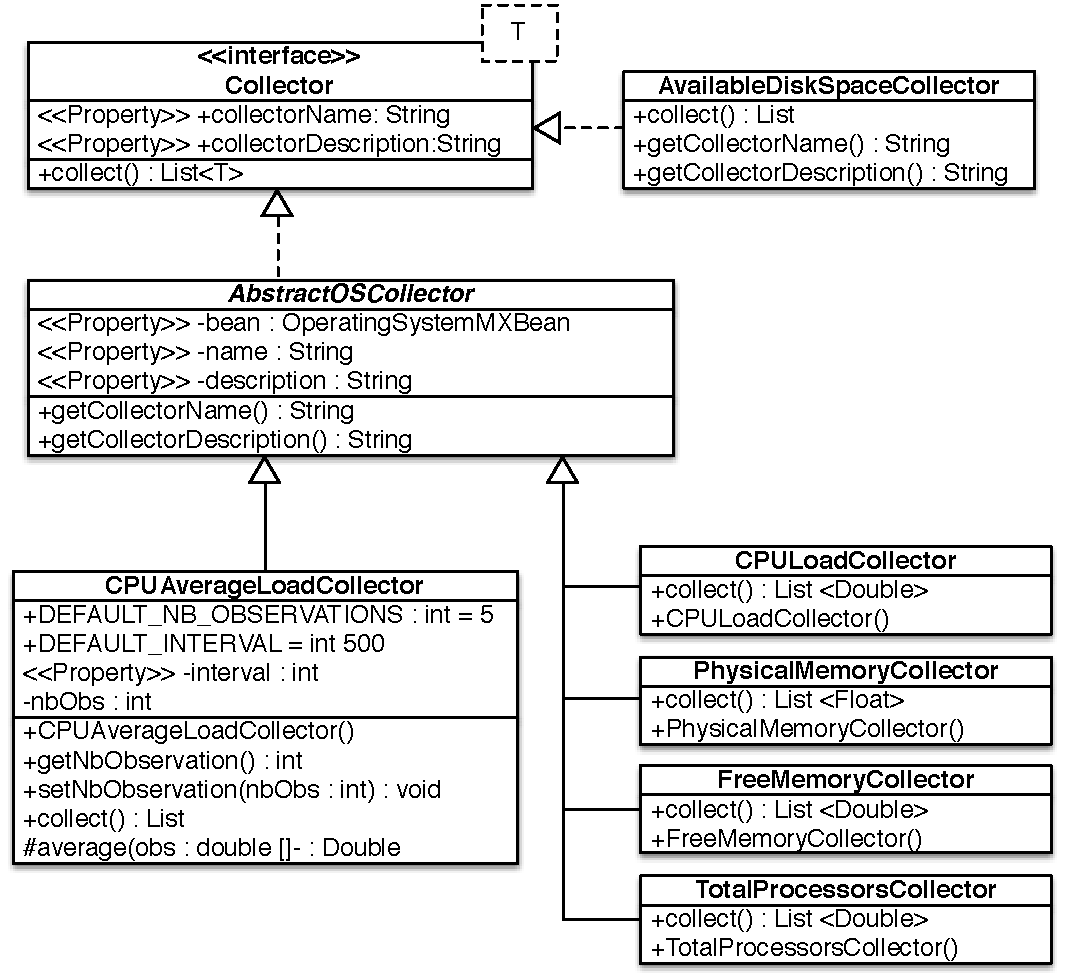
\includegraphics[width=15cm]{figuras/CollectorUML2.pdf}
   \caption{Diagrama de classes dos coletores de contexto}
   \label{fig:collectorUML}
\end{figure}

Cada instância de Node Manager possui um conjunto de coletores (um para memória e um para processadores), os quais realizam a coleta num intervalo pré-definido. Os coletores são executados por uma \textit{thread} independente e possuem um intervalo de 30 segundos entre as coletas para não causar sobrecarga ou interrupção no  processamento das tarefas \textit{Map} e \textit{Reduce}.

%-------------------------------------------------------------------
\section{Comunicação Distribuída}
\label{sec:zookeeper}

Para que a informação coletada pelos coletores de contexto possa afetar o escalonamento é necessário que exista uma maneira para os Node Managers transmitirem os dados atualizados ao escalonador, a ferramenta escolhida para esta tarefa foi o ZooKeeper.

\subsection{ZooKeeper}
O ZooKeeper é um projeto da Apache e fornece ferramentas eficientes, confiáveis e tolerantes à falha para a coordenação de sistemas distribuídos \cite{Hunt2010}. Inicialmente, o ZooKeeper foi implementado como um componente do Hadoop e virou um projeto próprio conforme cresciam suas funcionalidades e sua utilização em outras aplicações. 

A arquitetura utilizada no ZooKeeper é a de cliente-servidor, sendo o servidor o próprio ZooKeeper (chamado de \textit{ensamble}), enquanto a aplicação que o está utilizando assume o papel de cliente. Os dados do ZooKeeper ficam armazenados em \textit{zNodes}, abstrações que podem ser tanto um \textit{container} de dados quanto de outros \textit{zNodes}, e formam um sistema de arquivos hierárquico que pode ser comparado à estrutura de uma árvore. Para garantir a consistência deste sistema de arquivos o ZooKeeper utiliza operações de escrita linearizáveis, as quais são obrigatoriamente processadas pelo servidor líder que é, então, encarregado de propagar as mudanças para os demais participantes do \textit{ensamble} \cite{Pham}.

Um dos principais recursos do ZooKeeper são os \textit{Watchers}, interfaces providas pelo \textit{framework} que permitem aos clientes monitorarem certos \textit{zNodes}. Quando um \textit{Watcher} é registrado como monitor de um \textit{zNode}, ele pode ser configurado para monitorar a alteração dos dados do \textit{zNode}, a criação/remoção de \textit{zNodes} filhos, ou ainda para qualquer tipo de alteração no \textit{zNode} e seus filhos. Quando um \textit{zNode} sofre uma alteração que o \textit{Watcher} está monitorando uma \textit{callback} é disparada para que o cliente faça o processamento desejado \cite{HadoopBook}.

No âmbito deste trabalho, os serviços do ZooKeeper são utilizados para monitorar as informações de contexto coletadas nos nós escravos e transmiti-las para o escalonador. Sendo que a comunicação é feita através de processos que atualizam e monitoram o conteúdo de \textit{zNodes}.

%----------------------
\subsection{Implementação}
A flexibilidade oferecida através dos \textit{zNodes}, permite que qualquer estrutura de dado seja inserida como informação. Optou-se por utilizar uma Tabela Hash, o que permite realizar a tarefa com apenas um \textit{zNode} e possibilita aos Node Managers a inserção das informações e ao escalonador o monitoramento de maneira simples.

Na solução adotada há apenas um Watcher, o escalonador, que monitora o \textit{zNode} da Tabela Hash. Qualquer alteração na tabela dispara uma \textit{callback} no escalonador, que por sua vez percorre a tabela à procura das modificações e realiza as alterações pertinentes nas informações sobre os recursos. Esta abordagem permite que o escalonador realize operações apenas quando necessário e não desperdice tempo acessando a tabela quando não houverem atualizações a fazer.
A estrutura adotada no trabalho podes ser visualizada na Figura \ref{fig:zk}.
%Uma discussão possível de ser feita é sobre a decisão de utilizar somente 1 \textit{zNode} para toda tabela e o impacto disto em um cluster de 100 nós ou mais. Seria possível utilizar 1 \textit{zNode} para cada Node Manager, porém isto poderia fazer com que as \textit{callbacks} se acumulassem e o escalonador teria muitos processos apenas para atualizar os dados, uma vez que cada atualização geraria uma callback.

\begin{figure}[!hbtn]
   \centering
   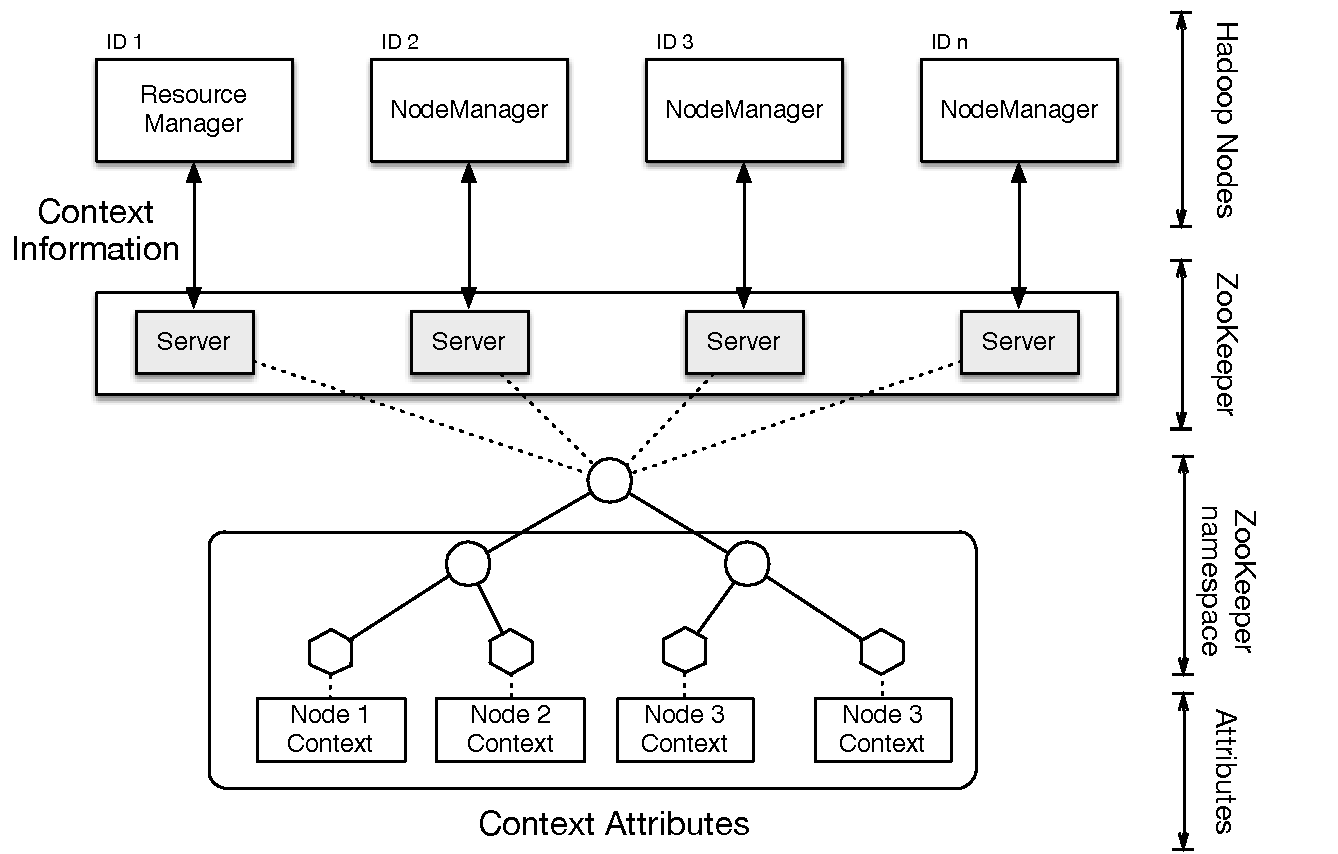
\includegraphics[width=15cm]{figuras/Zookeeper.pdf}
   \caption{Estrutura do ZooKeeper}
   \label{fig:zk}
\end{figure}

Como a solução escolhida apresenta dois papéis de clientes ZooKeeper, a seguir encontra-se uma explicação aprofundada de cada um destes papéis.

\begin{itemize}
	\item Cliente de Monitoramento: o papel de monitor é desempenhado pelo escalonador. O escalonador implementa a interface Watcher, fornecida pelo ZooKeeper, e monitora o \textit{zNode} que contém a Tabela Hash. No momento da inicialização o escalonador cria um \textit{zNode} e insere uma Tabela Hash vazia como informação, então finalmente, inicia o monitoramento do \textit{zNode}. Quando a \textit{callback} é acionada, a \textit{thread} percorre a tabela em busca de qual informação foi atualizada, atualiza os dados do escalonador e reinicia o monitoramento.
	
	\item Clientes de Atualização: o papel de atualização é realizado pelos Node Managers. Cada Node Manager lança, no momento de sua inicialização, uma \textit{thread} que faz a coleta de dados e caso haja alteração com relação à ultima leitura insere os dados atualizados na tabela hash. A coleta dos dados é realizada a cada 30 segundos, média de tempo observada em \textit{containers} executados em um \textit{cluster} de funcionamento normal. Para evitar o envio de dados por alterações naturais do sistema e que não impactariam o escalonamento foi implementado um \textit{threshold} mínimo de alteração de 100 Mb e/ou 1 \textit{core}.
	
\end{itemize}

%-------------------------------------------------------------------
\section{Solução Implementada}
\label{sec:solucao}
O Capacity Scheduler já possui adaptabilidade à entrada de novos Node Managers no cluster desde que um dos arquivos XML do Resource Manager tenha o \textit{host} do novo manager incluído e o Node Manager seja inicializado.
%TODO descrever geral,
%TODO colocar imagem da solução

\subsection{Integração dos Coletores de Contexto}
%TODO explicar como os coletores são inseridos na aplicação

\subsection{Integração dos Clientes}
%TODO explicar como os clientes zk interagem

\subsection{Justificativas para }